\documentclass[border=8pt]{standalone}
\usepackage{fontspec}
\defaultfontfeatures{Ligatures=TeX}
\setmainfont{Palatino Linotype}
\setsansfont{Arial}
\usepackage{amsmath,amssymb}
\usepackage{tikz}
\usetikzlibrary{arrows.meta,positioning,calc,shapes.geometric,fit}
\definecolor{tksInk}{HTML}{1C1A16}
\definecolor{tksMuted}{HTML}{8A8378}
\definecolor{tksAccent}{HTML}{8C5A1F}
\definecolor{tksAfill}{HTML}{F6EEDD}
\definecolor{tksAedge}{HTML}{9A7328}
\definecolor{tksBfill}{HTML}{E6EDF5}
\definecolor{tksBedge}{HTML}{2F5B85}
\definecolor{tksCfill}{HTML}{F7E7E4}
\definecolor{tksCedge}{HTML}{95403A}
\definecolor{tksDfill}{HTML}{E4EFE6}
\definecolor{tksDedge}{HTML}{3A6B45}
\definecolor{tksEfill}{HTML}{F5DFDC}
\definecolor{tksEedge}{HTML}{A33B30}
\begin{document}
\centering
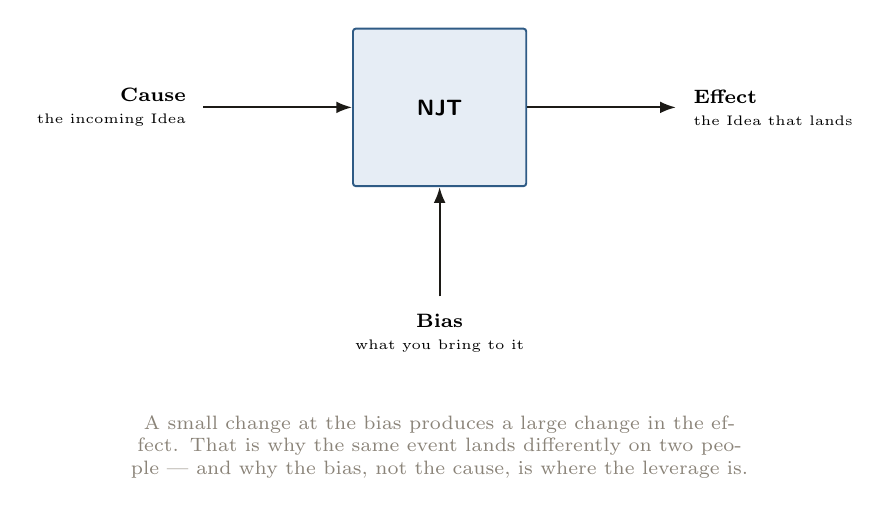
\begin{tikzpicture}[x=1mm, y=1mm, font=\sffamily\footnotesize]
  \node[rounded corners=1pt, minimum width=22mm, minimum height=20mm,
        fill=tksBfill, draw=tksBedge, line width=0.7pt] (n) at (0,0)
        {\textbf{NJT}};
  \draw[-{Latex[length=2mm]}, tksInk, line width=0.7pt] (-30,0) -- (n.west);
  \node[anchor=east, align=right, font=\scriptsize] at (-31,0)
    {\textbf{Cause}\\{\tiny the incoming Idea}};
  \draw[-{Latex[length=2mm]}, tksInk, line width=0.7pt] (0,-24) -- (n.south);
  \node[anchor=north, align=center, font=\scriptsize] at (0,-25)
    {\textbf{Bias}\\{\tiny what you bring to it}};
  \draw[-{Latex[length=2mm]}, tksInk, line width=0.7pt] (n.east) -- (30,0);
  \node[anchor=west, align=left, font=\scriptsize] at (31,0)
    {\textbf{Effect}\\{\tiny the Idea that lands}};
  \node[anchor=north, text width=92mm, align=center, font=\scriptsize,
        text=tksMuted] at (0,-38)
    {A small change at the bias produces a large change in the effect. That is
     why the same event lands differently on two people --- and why the bias,
     not the cause, is where the leverage is.};
\end{tikzpicture}
\end{document}
